\documentclass[12pt]{article}

\usepackage{amsmath, mathtools}
\usepackage{amsfonts}
\usepackage{amssymb}
\usepackage{graphicx}
\usepackage{colortbl}
\usepackage{xr}
\usepackage{longtable}
\usepackage{xfrac}
\usepackage{siunitx}
\usepackage{tabularx}
\usepackage{float}
\usepackage{booktabs}
\usepackage{caption}
\usepackage{pdflscape}
\usepackage{afterpage}
\usepackage{calc}
\usepackage{multirow}
\usepackage{array}
\usepackage{longtable}
\usepackage{rotating}

\usepackage[a4paper]{geometry}
\usepackage[acronym,nomain,section=section,numberedsection]{glossaries}
\usepackage[round]{natbib}
\usepackage[bookmarks=true,breaklinks]{hyperref}

%% Comments

\usepackage{color}

\newif\ifcomments\commentstrue %displays comments
%\newif\ifcomments\commentsfalse %so that comments do not display

\ifcomments
\newcommand{\authornote}[3]{\textcolor{#1}{[#3 ---#2]}}
\newcommand{\todo}[1]{\textcolor{red}{[TODO: #1]}}
\else
\newcommand{\authornote}[3]{}
\newcommand{\todo}[1]{}
\fi

\newcommand{\wss}[1]{\authornote{blue}{SS}{#1}} 
\newcommand{\plt}[1]{\authornote{magenta}{TPLT}{#1}} %For explanation of the template
\newcommand{\an}[1]{\authornote{cyan}{Author}{#1}}

%% Common Parts

\newcommand{\progname}{MECHTRON 4TB6} % PUT YOUR PROGRAM NAME HERE
\newcommand{\authname}{Group 1, UWheeledChair,
\\ Lisa Ji
\\ Haoyu Lin
\\ Yuntian Wang
\\ Zichun Yan } % AUTHOR NAMES                  

\usepackage{hyperref}
    \hypersetup{colorlinks=true, linkcolor=blue, citecolor=blue, filecolor=blue,
                urlcolor=blue, unicode=false}
    \urlstyle{same}
% \hypersetup{
%     colorlinks=true,       % false: boxed links; true: colored links
%     linkcolor=red,          % color of internal links (change box color with linkbordercolor)
%     citecolor=green,        % color of links to bibliography
%     filecolor=magenta,      % color of file links
%     urlcolor=cyan           % color of external links
% }

% For easy change of table widths
\newcommand{\colZwidth}{1.0\textwidth}
\newcommand{\colAwidth}{0.13\textwidth}
\newcommand{\colBwidth}{0.82\textwidth}
\newcommand{\colCwidth}{0.1\textwidth}
\newcommand{\colDwidth}{0.05\textwidth}
\newcommand{\colEwidth}{0.8\textwidth}
\newcommand{\colFwidth}{0.17\textwidth}
\newcommand{\colGwidth}{0.5\textwidth}
\newcommand{\colHwidth}{0.28\textwidth}

\makenoidxglossaries
    \newlength\maxlength
    \newlength\thislength
    \newglossarystyle{mystyle}
    {%
      \renewenvironment{theglossary}%
      {% start of glossary
       % Find maximum width of the first column:
        \setlength{\maxlength}{0pt}%
        \forglsentries[\currentglossary]{\thislabel}%
        {%
           \settowidth{\thislength}{\glsentryshort{\thislabel}}%
           \ifdim\thislength>\maxlength
             \setlength{\maxlength}{\thislength}%
           \fi
        }%
        % Now calculate the width of the second column:
        \settowidth{\thislength}{\hspace{1.5em}=\hspace{1em}}%
        \setlength{\glsdescwidth}{\linewidth-\maxlength-\thislength-2\tabcolsep}%
        % Start the tabular environment
        \begin{tabular}{l@{\hspace{1.5em}=\hspace{1em}}p{\glsdescwidth}}
        \toprule
        \multicolumn{1}{l}{\textbf{symbol}} &
        \multicolumn{1}{@{}l}{\textbf{description}}\\%
        \midrule
      }%
      {% end of glossary
         \bottomrule
         \end{tabular}%
      }%
      % Header has been incorporated into \begin{theglossary}
      \renewcommand*{\glossaryheader}{}%
      % Don't do anything between letter groups
      \renewcommand*{\glsgroupheading}[1]{}%
      \renewcommand*{\glsgroupskip}{}%
      % Set display for each the acronym entry
      \renewcommand{\glossentry}[2]{%
        \glstarget{##1}{\glsentryshort{##1}}% short form
        &
        \glsentrylong{##1}% long form
        \\% end of row
      }%
      % No sub-entries, so \subglossentry doesn't need redefining
    }
\newacronym{wbr}{WBR}{Wheeled Bipedal Robot}
\newacronym{har}{HAR}{Hazard Analysis Report}
\newacronym{imc}{IMC}{Inter-Module Communication}
\newacronym{ca}{CA}{Critical Assumptions}
\newacronym{emi}{EMI}{Electro Magnetic Interference}
\newacronym{imu}{IMU}{Inertial Measurement Unit}
\newacronym{lidar}{LiDAR}{Light Detection and Ranging}
\newacronym{crc}{CRC}{Cyclic Redundancy Check}
\newacronym{srs}{SRS}{System Requirements Specification}
\newacronym{assump}{A}{Assumption}
\newacronym{dd}{DD}{Data Definition}
\newacronym{gd}{GD}{General Definition}
\newacronym{gs}{GS}{Goal Statement}
\newacronym{im}{IM}{Instance Model}
\newacronym{lc}{LC}{Likely Change}
\newacronym{ps}{PS}{Physical System Description}
\newacronym{req}{R}{Requirement}
\newacronym{theo}{T}{Theoretical Model}
\newacronym{macrm}{MacRM}{MacRobomaster Club}
\newacronym{com}{CoM}{Center of Mass}
\newacronym{na}{N/A}{Not Applicable}
\newacronym{dji}{DJI}{SZ DJI Technology Co., Ltd.}
\newacronym{rmul}{RMUL}{RoboMaster University League}
\newacronym{fsm}{FSM}{Finite State Machine}
\newacronym{tbd}{TBD}{To be declared}
\newacronym{pid}{PID}{Proportional–integral–derivative}

% Used so that cross-references have a meaningful prefix
\newcounter{defnum} %Definition Number
\newcommand{\dthedefnum}{GD\thedefnum}
\newcommand{\dref}[1]{GD\ref{#1}}
\newcounter{datadefnum} %Datadefinition Number
\newcommand{\ddthedatadefnum}{DD\thedatadefnum}
\newcommand{\ddref}[1]{DD\ref{#1}}
\newcounter{theorynum} %Theory Number
\newcommand{\tthetheorynum}{T\thetheorynum}
\newcommand{\tref}[1]{T\ref{#1}}
\newcounter{tablenum} %Table Number
\newcommand{\tbthetablenum}{T\thetablenum}
\newcommand{\tbref}[1]{TB\ref{#1}}
\newcounter{assumpnum} %Assumption Number
\newcommand{\atheassumpnum}{P\theassumpnum}
\newcommand{\aref}[1]{A\ref{#1}}
\newcounter{goalnum} %Goal Number
\newcommand{\gthegoalnum}{P\thegoalnum}
\newcommand{\gsref}[1]{GS\ref{#1}}
\newcounter{instnum} %Instance Number
\newcommand{\itheinstnum}{IM\theinstnum}
\newcommand{\iref}[1]{IM\ref{#1}}
\newcounter{reqnum} %Requirement Number
\newcommand{\rthereqnum}{P\thereqnum}
\newcommand{\rref}[1]{R\ref{#1}}
\newcounter{lcnum} %Likely change number
\newcommand{\lthelcnum}{LC\thelcnum}
\newcommand{\lcref}[1]{LC\ref{#1}}

\newacronym{slam}{SLAM}{Simultaneous Localization and Mapping. A technique that allows the robot to create a map of its surroundings and estimate its own position within the map}
\glsadd{slam}
\newacronym{ui}{UI}{User Interface. A software program that allows the user to interact with the robot and the delivery system.}
\glsadd{ui}
\newacronym{ctrl}{CTRL}{The main embedded system controller. It receives command from MiniPC to control the fundamental actuator system. Overall, it control the WBR posture and movement.}
\glsadd{ctrl}
\newacronym{minipc}{MiniPC}{A mini computer that receives user input, handles image processing and SLAM, to make decisions and send the decisions to CTRL}
\glsadd{minipc}
\newacronym{jump}{Jump Mode}{A controller mode make the robot to jump over obstacles or gaps.}
\glsadd{jump}

\title{Project Deliverable Contract\\\progname}
\author{\authname}
\date{\today}

\begin{document}

\maketitle
\pagenumbering{arabic}

\newpage
\begin{table}[hp]
    \caption{Revision History} \label{TblRevisionHistory}
    \begin{tabularx}{\textwidth}{llX}
        \toprule
        \textbf{Date} & \textbf{Developer(s)}    & \textbf{Change} \\
        \midrule
        2023-11-25    & Lisa Ji, Haoyu Lin       & Revision 0      \\
                      & Yuntian Wang, Zichun Yan &                 \\
        \bottomrule
    \end{tabularx}
\end{table}

\newpage
\tableofcontents
\listoftables
\listoffigures

\printnoidxglossary[type=\acronymtype,style=mystyle,title=Naming Conventions and Terminology]

\newpage
\section{Introduction}
\subsection{Document Purpose} \label{sec:Document Purpose}
This document provides deliverable contract for the UWheeledChair project of Group 1. It outlines the essential deliverable for the project, and will serve as a basis for evaluating the completion of the project. The whole documentation is divided into three parts: Delivery Control Deliverables, Robot Control Deliverables and Evaluation Criteria.
\subsection{Project Purpose} \label{sec:Project Purpose}
\begin{figure}[H]
    \centering
    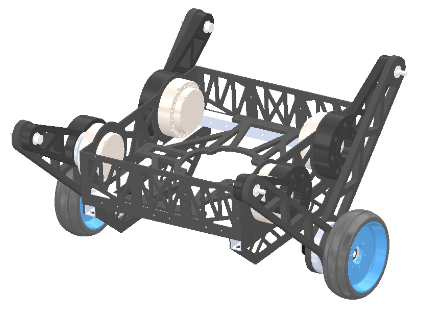
\includegraphics[scale=0.7]{../Mechanical Platform.png}
    \caption{\acrshort{wbr} Mechanical Platform}
    \label{fig:Mechanical Platform}
\end{figure}
This project is to develop the software and control system for a fully-autonomous delivery robot, based on the existing assembly of a \acrfull{wbr} provided by the \acrfull{macrm}, as shown in Figure \ref{fig:Mechanical Platform}. The project will be referred to as the \acrshort{wbr} project in the following documents.\\\\
For \acrshort{macrm}, \acrshort{wbr} was constructed following the constraints defined in the rules, \citet{RmuBuildSpecs2024}, of the 2024 \acrfull{rmul} Competition, whose host is \acrfull{dji}. Details of the constraints is shown in section Design Constraints of another document, the \gls{srs}.\\\\
Since the mechanical and electronic hardware are fixed constraints, the \acrshort{wbr} project mainly focuses on the software and control system, while the \acrshort{macrm} is responsible for the mechanical design, provision, and maintenance.

\section{Delivery Control Criteria}
    The delivery control system as operated by \acrshort{minipc} is responsible for the high level decision-making functionality of the robot, whose overall goal to deliver parcels from a delivery station to a destination.
    \subsection{SLAM}
        \begin{itemize}
            \item Able to read and process information from sensors (such as cameras, \acrshort{lidar}, \acrshort{imu}, etc.) in at least 10 Hz frequency.
            \item Able to accurately locate robot itself in a given environment with less than 0.1 m error compared to ground truth after running at least 20 minutes.
            \item Able to detect unexpected local obstacles at least 3 meters ahead.
        \end{itemize}
    \subsection{Path Tracking and Finding}
        \begin{itemize}
            \item Able to find a suitable path from the delivery station to the destination using a pre-defined map or a SLAM-generated map
            \item Able to return to the delivery station after the parcel is being picked up.
            \item Able to constantly gather information from SLAM and update paths related to unexpected local obstacles.
            \item Able to restrict the robot to stay in designated areas.
        \end{itemize}
    \subsection{User Communication}
        \begin{itemize}
            \item Able to allow the sender to schedule delivery tasks and assign destinations using a \acrshort{ui}.
            \item Able to notify the sender and the receiver when the robot arrives at the destination.
        \end{itemize}     
    \subsection{Parcel Handling}
        \begin{itemize}
           \item Able to allow sender to load parcel and receiver to take parcel out only with given credentials.
            \item (Optional Criterion) Parcel Status Monitoring: able to monitor and display the status of the parcel, such as weight, temperature, humidity, etc. The box should be able to notify the sender and the receiver if the parcel status exceeds the acceptable range.
        \end{itemize}

\section{Robot Control Criteria}
The control criteria system is responsible for the stability and agility of the robot, which are essential for the delivery performance.
    \subsection{Posture Control}
        \begin{itemize}
            \item Able to respond to user commands quickly, including roll, pitch, and yaw angle adjustment of the package platform.
            \item Able to maintain the body posture stably upright.
            \item Able to recover the body posture after external disturbance, for example, a slight kick by a human.
        \end{itemize}
    \subsection{Motion Control}
        \begin{itemize}
            \item Able to move at constant speeds, the maximum speed should be at least 1 m/s.
            \item Able to rotate at constant speeds, the maximum speed should be at least 30 rpm.
            \item Able to do a sharp turn, the minimum turning radius should be at most as wide as two robot bodies at the moving speed of 1 m/s.
        \end{itemize}
    \subsection{Jump Control}
        \begin{itemize}
            \item Able to jump high enough that the robot can stay floating in air for at least 0.4 seconds.
            \item Able to launch jump from an asymmetric terrain, where the initial state of the robot chassis platform is not possible to be horizontal.
            \item Able to jump across a 0.25 m wide chasm.
            \item Able to jump consecutively at least twice while moving or rotating the robot body
        \end{itemize}

\section{Evaluation Criteria}
The completion of the project will be evaluated based on the successful implementation and functioning of the above-listed deliverables. Each deliverable must meet its described criteria to be considered complete. The evaluation will be conducted by testing the robot in a simulated or real environment, and measuring its performance using various metrics such as accuracy, speed, reliability, etc.

\newpage
\section{Appendix A - Table of Units}
Throughout this document SI (Syst\`{e}me International d'Unit\'{e}s) is employed
as the unit system.  In addition to the basic units, several derived units are
used as described below.  For each unit, the symbol is given followed by a
description of the unit and the SI name.
~\newline

\renewcommand{\arraystretch}{1.2}
%\begin{table}[ht]
\noindent \begin{tabular}{l l l}
    \toprule
    \textbf{symbol}    & \textbf{unit}   & \textbf{SI}                       \\
    \midrule
    \si{\metre}        & length          & metre                             \\
    \si{\kilogram}     & mass            & kilogram                          \\
    \si{\second}       & time            & second                            \\
    \si{\minute}       & time            & minute                            \\
    % \si{\celsius}      & temperature     & centigrade                        \\
    % \si{\joule}        & energy          & Joule                             \\
    % \si{\watt}         & power           & Watt (W = \si{\joule\per\second}) \\

    \si{m/s}           & speed           & meter/second                      \\
    m/s$^2$            & acceleration    & meter per second square           \\
    % \si{\ampere\hour}  & electric charge & ampere hour                       \\
    % cm                 & length          & centimeter                        \\
    % \si{\volt}         & voltage         & volt                              \\
    % \si{\newton\meter} & torque          & newton per meter                  \\
    rpm & angular speed          & round per minute                  \\
    Hz       & frequency           & times per second                            \\
    % \si{\radian}       & angle           & radian                            \\

    \bottomrule
\end{tabular}
%	\caption{Provide a caption}
%\end{table}

\newpage
\bibliographystyle {plainnat}
\bibliography {../References}

\end{document}